\chapter{Chosen Application Architecture}

\section{Proposed Architecture}
After researching available technologies, an architecture to build the pfcrender tool on was selected. The implementation is shown alongside the original requirements in the following graphs, split between functional- (figure \ref{fr}) and non-functional (figure \ref{nfr}) requirements. As before, direct requirements are highlighted in green. Take note that each direct requirement is satisfied or verified through an implementation requirement or test case.

The architecture is discussed in detail in the following sections.

\begin{figure}[p]
	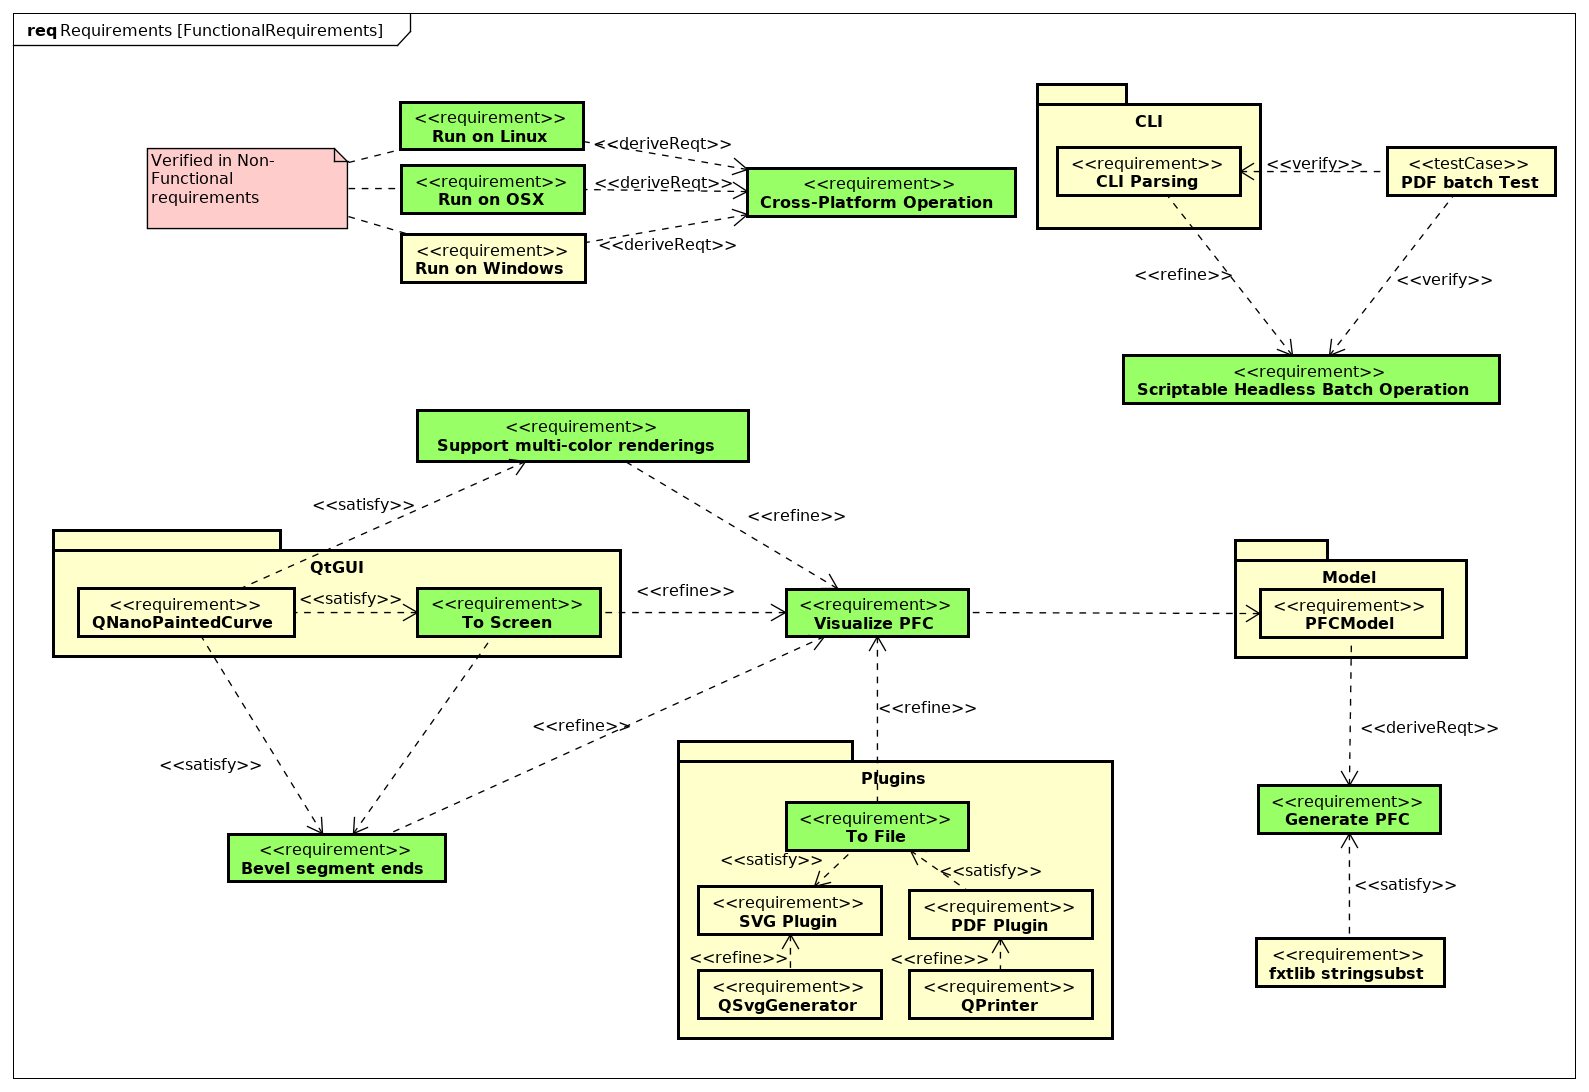
\includegraphics[width=\textwidth]{FunctionalRequirements}
	\caption{Functional requirements}
	\label{fr}
\end{figure}

\begin{figure}[p]
	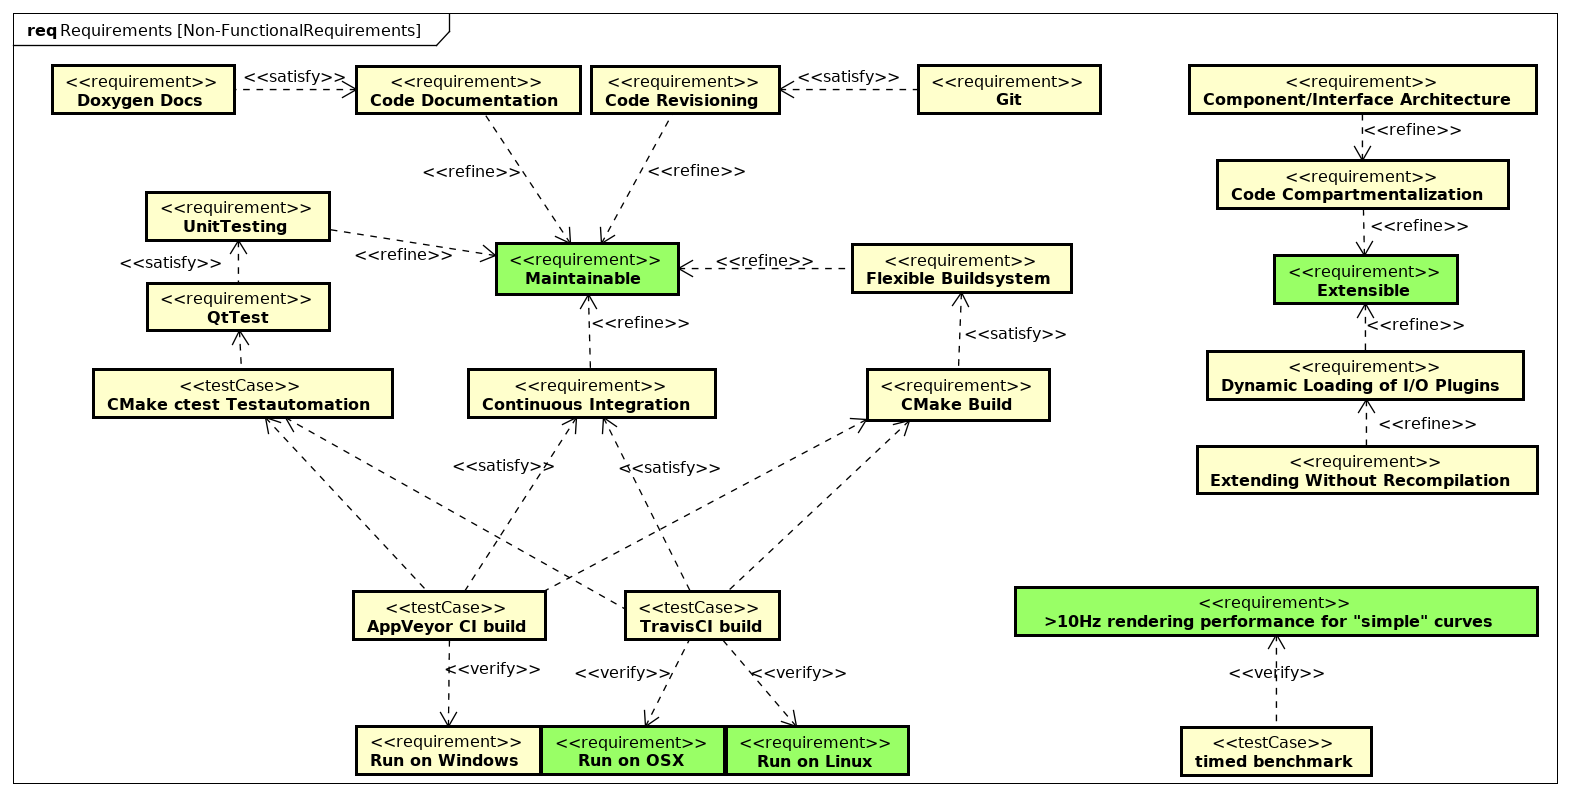
\includegraphics[width=\textwidth]{Non-FunctionalRequirements}
	\caption{Non-functional requirements}
	\label{nfr}
\end{figure}

\subsection{Functional Requirements}
The main decision to make on the software architecture side was which of the framework libraries discussed in section \ref{sec:res_frameworks} to use.
This was mainly driven by three main concerns: extensibility, performance and ease-of-use.

Ultimately, the Qt Framework was chosen for the following reasons:
\begin{itemize}
	\item Platform-independent dynamic library loading abstraction provided, which is useful for implementing the plugin architecture described in \ref{sec:pluginarch}
	\item Classes provided for exporting e.g. to SVG and PDF
	\item Though Qt is not a light-weight framework like \gls{sdl}, 2D rendering performance should be good enough when rendering via the QtQuick \gls{api} (see \ref{asomewhere})
	\item Multiple quality-of-life improvements like the QtCreator \gls{ide} with \gls{gui} designer
	\item Included QtTest Unit-Testing Framework
\end{itemize}

Qt provides most of the wanted features in one framework, keeping additional dependencies to a minimum. One notable exception is the drawing \gls{api}, which proved unsuitable during implementation and resulted in inclusion of an additional module (see \ref{sec:qnanopainter}). 

A description of the Qt provided mechanisms used in this tool follows

\subsubsection{Dynamic Library Loading}
Windows DLL API mandates symbols callable from outside a library to be prefixed with a macro on export and import. The \gls{msdn}\furl{https://msdn.microsoft.com/en-us/library/3y1sfaz2.aspx} defines it the following way
\begin{lstlisting}
__declspec( dllimport ) declarator  
__declspec( dllexport ) declarator  
\end{lstlisting}

Linux compilers like gcc will not be able to parse this keyword and fail compilation. While it is possible to work around this issue by wrapping the keyword in a preprocessor macro that expands to nothing on Linux, this mechanism is cumbersome to implement.

To get cross-\gls{os} operation without recompiling, use Qt's Library loading mechanism: QPluginLoader OR QLibrary.

This adds an additional step of making Qt's MetaObjectSystem aware of the library but avoids OS-specific switches/preprocessor macros

\subsubsection{Rendering in Qt}
As stated before, Qt offers two different application programming \gls{api}s. A main difference is in the rendering methode they use:
\begin{description}
	\item [QWidgets] The main API of Qt. It is Java SWING-like and handles GUI design and functionality in C++ using Qt-provided or custom QWidget-derived classes.
	\item [QtQuick] A relatively new (since Qt 4.7) javascript-based declarative language called \gls{qml}, similar to the XML-based JavaFX, is used to define the GUI frontend, while C++ classes in the backend are used for performance intensive calculation. The UI is then rendered in a so-called scenegraph using a platform specific graphics backend like OpenGL or OpenGL ES. Though no formal study of performance differences between both \gls{api}s exists, documentation by the QtCompany\furl{http://doc.qt.io/qt-5/qtquick-performance.html} suggests performance between both models is comparable if some guidelines are followed.
\end{description}

Since the additional model-/view abstraction is very conducive to extensibility, as the declarative nature makes extending the UI easy, QtQuick is selected for the implementation.


The following methods of drawing to these APIs are offered:
\begin{description}
	\item [QPainter] Oldest drawing API of Qt, used in QWidgets. Not directly usable in QtQuick. Offers highest amount of integration to other Qt classes (notably QPrinter and QSVGGenerator)
	\item [QtQuick/QML shape] Placing line segments directly in a \gls{qml} file and loading it to the SceneGraph (creating quadratic bezier curves added in Qt 5.10 (late 2017), too late for this work\furl{https://blog.qt.io/blog/2017/08/10/let-there-be-more-shapes/})
	\item [QtQuick HTML5 canvas] Draws on top of a HTML5 canvas embedded into the qt app.
	\item [QtQuick Item with custom scene graph node] Instantiates a QQuickItem with a custom appearance by setting vertices and material directly\todo{explain what those are}
	\item [QQuickPaintedItem] An adaptation of the QPainter API for the SceneGraph based QtQuick. 
	\item [QNanoPainter] A third party plugin, offering a mixture of QPainter and HTML5 canvas API to draw on an OpenGL framebuffer object to be placed in the QtQuick scene graph. Offers Painter-like productivity with less performance overhead.
\end{description}

The QML and HTML5 APIs were disregarded due to their interpreted and thus slow nature.

This leaves direct QuickItem implementation, QQuickPaintedItem and QNanoPainter-based QuickItem as viable options.

Due to performance measurements\furl{https://www.vikingsoftware.com/qtquick-custom-item-performance/}, a direct implementation was chosen intially (see \ref{somewhere}). The operations performed using this \gls{api} were too inflexible to allow for generation of quadratic bézier curves necessary to implement rounded edges (see \ref{somewhere}), so a higher level \gls{api} was selected.

Further performance benchmarks\furl{http://kgronholm.blogspot.com/2017/12/qt-510-rendering-benchmarks.html} led to preferring QNanoPainter over the built-in QQuickPaintedItem, even though it meant introducing an additional dependency into the project.

It is worth noting, that QPainter \gls{api} was still used for file outputs (see \ref{svg}, \ref{pdf}), where performance is not as critical, due to its integration with other Qt exporter classes.

\subsection{Qt Unit Testing Framework}

Qt comes with its own unit-testing framework integrated into QtCreator. The following example is an example test for a fictional Counter class:

\begin{lstlisting}
#include <QtTest>
#include "Counter.h"

class MyTest : public QObject {
    Q_OBJECT

    Counter* ctr;

private slots:
    void initTestCase();

    void do_count();
  //void do_downcount(); // additional test routines

    void cleanupTestCase();
};

void MyTest::initTestCase()
{
	ctr = new Counter(0);
}

void MyTest::cleanupTestCase()
{
    delete ctr;
}

void MyTest::do_count()
{
	ctr->count();
	QVERIFY(ctr->getValue() == 1);
}

QTEST_MAIN(MyTest)
#include "MyTest.moc"
\end{lstlisting}

This builds an executable (main routine provided by the QTEST\_MAIN macro) that runs the given test routines.
It is integrated with QtCreator, which gathers test apps created in this way automatically and can run them from the \gls{gui} and display PASS/FAIL status depending on QVERIFY() and return value.
\begin{figure}[h]
	\todo{qtcreatbild}
\end{figure}

Since it is a standalone executable, it can also be run by other testing environments like CMake's CTest, and can thus be automated and integrated into \gls{ci} builds.

\begin{figure}[h]
	\todo{travis buildlog}
\end{figure}

\section{Flexible Buildsystem}
Though as described in \ref{sec:somewhere} Qt has its own makefile generator with qmake, CMake was selected for this projects for the following reasons
\begin{itemize}
	\item CMake is more widely used in the \gls{floss} community
	\item It is more flexible in generators
	\item QtCreator has good CMake integration
\end{itemize}

Though it would surely be possible to have the platform agnosstic sources present, and then manually create a project for MSVC/MinGW when on Windows, gnu gcc on Linux and clang on Mac, this would be a pain to set up and maintain.

Solutions to this problem exist in so-called buildsystem generators. Those gather sources, dependencies and additional project information from a configuration file, detect the architecture they are running on, and generate the files necessary to compile the full project on whichever compiler is present on the current system.

QMake - The native buildsystem generator of Qt, uses .pro files for project description

CMake - A powerful and scalable config script-driven generator that is widely used in both Open Source and commercial projects 


\section{Commandline Parsing}
Unlike other programming languages (e.g. Python), C++ does not provide a standard built-in facility to provide parsing capability for parsing parameters passed to the program as commandline options.

Alternatives:

\begin{itemize}
\item getopt() - Coming from C, this is a legacy method widely used on Linux. Since it is specific to POSIX systems, it cannot be used on Windows 
\item Boost.progam\_options - A C++ native, highly configurable solution shipped with the open source Boost library
\url{http://www.boost.org/doc/libs/1\_58\_0/doc/html/program\_options.html}
\item QtCommandLineParser - A Qt native parsing class. Batch-parses all parameters and returns data structures with positional arguments in correct order, and a (reordered) map of switches with their parameters
http://doc.qt.io/qt-5/qcommandlineparser.html
\item Manual parsing of the argv array. While this is the most flexible solution in customization, it is reinventing the wheel and also very inflexible with respect to extensibility.
\end{itemize}

Due to it supporting our use-case, being easily extensible and not introducing any more dependencies into the project above the already used Qt Framework libraries, the QtCommandLineParser was chosen to provide the main CLI-based interface to the program.


\section{Option Persistency}
Since it is often unneccessary to set any and all config options for the program on the command line each time it is run, keeping config options persistently over program relaunches is useful. The typical implementation of this persistent store again varies by platform, ranging from putting keys into the Windows registry, over property list files on Mac to plain .ini or .cfg files on Linux.

Again, Qt comes with a wrapper around this platform disparity

\section{Class Hierarchy}
\begin{figure}[p]
	\todo{class diagrams}
\end{figure}
